\chapter{Primeri uporabe}


\section{Uporaba modula api\_wrapper}

Enostavno uporabo modula \verb|api_wrapper| s skriptnim delom programa Orange
prikazuje primer \ref{scripting_example}. V temu primeru pogledamo, kako
učinkovito lahko napovemo smrtnost otrok iz raznih indikatorjev zdravja,
okolja in infrastrukture. V vrsticah $5$ do $15$ naredimo poizvedbe po
potrebnih podatkih s programskega vmesnika Svetovne banke. Nato v vrsticah $18$
do $27$ odstranimo vrstice iz tabele, ki nimajo ciljne vrednosti in naredimo novo tabelo z
razredom, ki ga želimo napovedovati. Vrednosti, ki jih želimo napovedovati, se
nahajajo v stolpcu $55$ v tabeli \verb|class_data|. Ta stolpec vsebuje podatke
o smrtnosti otrok mlajših od enega leta za leto 2015. V naslednjih vrsticah
pa zgradimo tri napovedne modele: naključni gozd z
regresijskimi drevesi \verb|rf|, linearna regresija z regularizacijo 
\verb|ridge| in srednja vrednost \verb|mean|.
Za ocene napovednih modelov smo uporabili oceni
$RMSE$~\fnurl{https://en.wikipedia.org/wiki/Root-mean-square\_deviation} in 
$R^2$~\fnurl{https://en.wikipedia.org/wiki/Coefficient\_of\_determination}.
Rezultate primera \ref{scripting_example} lahko vidimo v tabeli 
\ref{rezultati_skripte}.


\begin{snippet}
\begin{center}
\lstinputlisting{example.py}
\end{center}
\cprotect
\caption{Napovedovanje smrtnosti otrok do enega leta iz podatkov o dostopnosti
  čiste vode, številu bolniških postelj na 1000 prebivalcev in odstotku
  cepljenih otrok do drugega leta starosti.}
\label{scripting_example}
\end{snippet} 

\begin{table}
\begin{center}

\begin{tabular}{l|r|r}
  Learner & RMSE & R2 \\ \hline
  rf & 9.74 & 0.79 \\
  ridge & 17.76 & 0.31 \\
  mean & 21.35 & -0.00
\end{tabular}
\end{center}
\cprotect
\caption{Rezultati napovedi smrtnosti otrok do enega leta starosti.}
\label{rezultati_skripte}
\end{table} 



\section{Napoved temperature s pomočjo $CO_2$ izpustov v ZDA}


Podatke svetovne banke lahko uporabimo tudi kot časovne vrste z uporabo
posebnih gradnikov za delo s časovnimi vrstami \cite{time_series}. Tukaj si
bomo ogledali enostaven primer napovedi temperature v ZDA s pomočjo podatkov o
izpustih $CO_2$. V tej napovedi smo uporabili podatke tako z gradnika 
WB Indicators (Slika \ref{var_indicator_select})
kot tudi z gradnika WB Climate (Slika \ref{var_climate_select}). Podatke obeh
gradnikov smo zdru"zili z gradnikom ``Merge Data'' po obeh "casovnih
komponentah. Nato smo odstranili vnose "casovnih obdobij za katere nimamo na
voljo vseh podatkov. Sestavljeno tabelo prikazuje slika \ref{var_data_table}.
Iz teh podatkov nato zgradimo "casovno vrsto in s pomočjo modela vektorske 
autoregresije VAR \cite{var_model} napovemo podatke za povprečno 
letno temperaturo za naslednjih nekaj let, kar je prikazano na sliki 
\ref{var_forecast_graph}.

\begin{figure}
\begin{center}
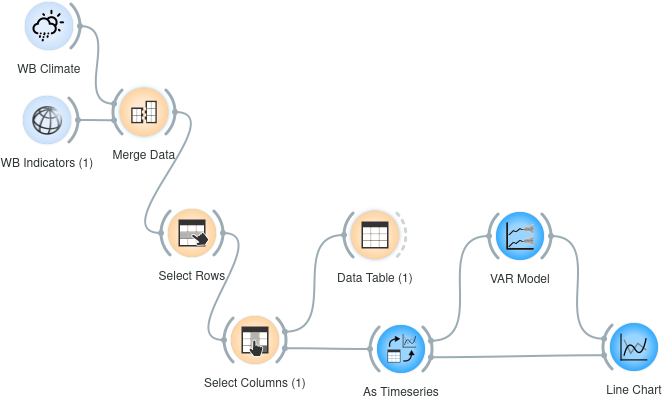
\includegraphics[width=11cm]{pic/var_setup.png}
\end{center}
\caption{Prikaz povezave gradnikov za napoved temperature.}
\label{var_setup}
\end{figure} 


\begin{figure}
\begin{center}
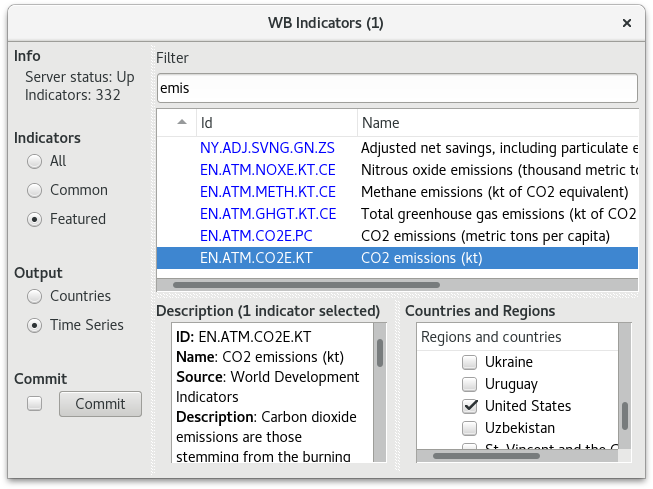
\includegraphics[width=12cm]{pic/var_indicator_select.png}
\end{center}
\caption{Izbor indikatorja $CO_2$ izpustov v ZDA.}
\label{var_indicator_select}
\end{figure} 

\begin{figure}
\begin{center}
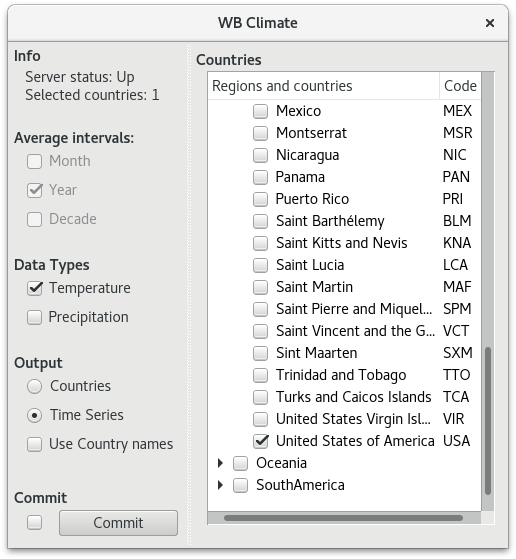
\includegraphics[width=8cm]{pic/var_climate_select.png}
\end{center}
\caption{Izbor podatkov povprečnih letnih temperatur v ZDA.}
\label{var_climate_select}
\end{figure} 

\begin{figure}
\begin{center}
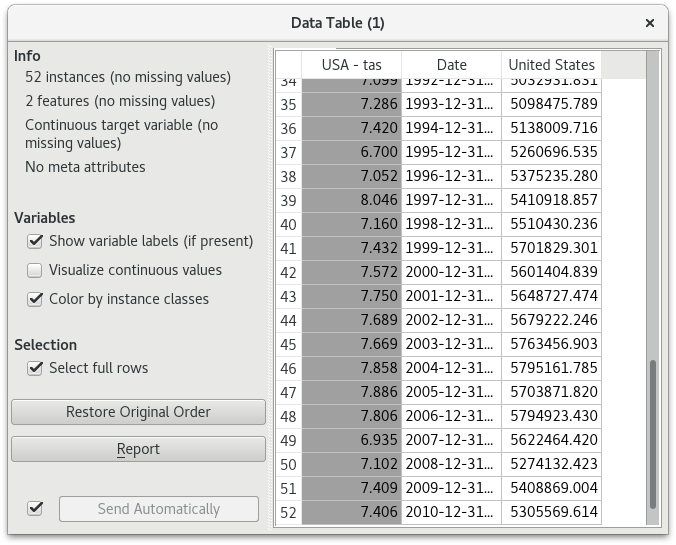
\includegraphics[width=10cm]{pic/var_data_table.png}
\end{center}
\caption{Podatkovna tabela s ciljnim razredom, in dvema poljema.}
\label{var_data_table}
\end{figure} 

\begin{figure}
\begin{center}
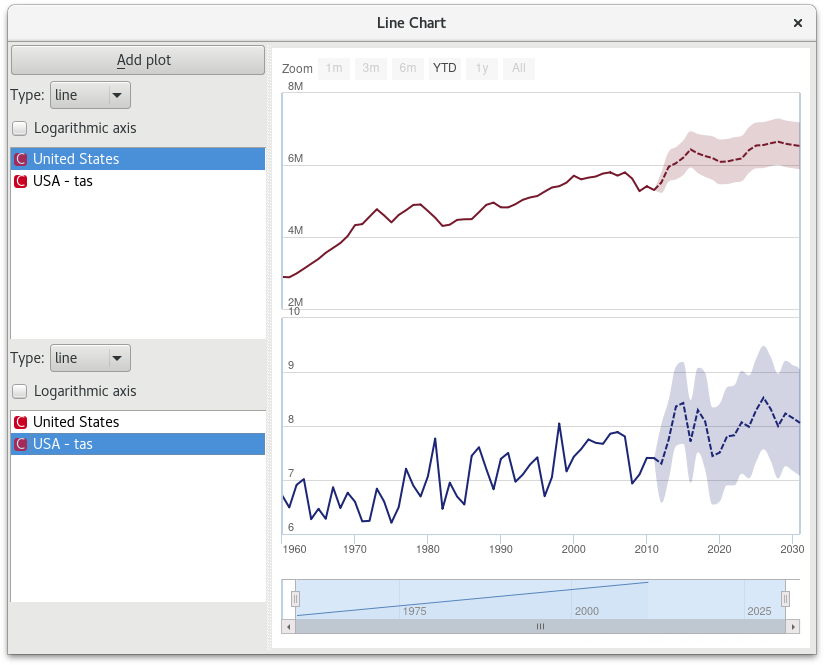
\includegraphics[width=12cm]{pic/var_forecast_graph.png}
\end{center}
\caption{Prikaz napovedi gibanja povprečnih letnih temperatur ``USA - tas'' in
  $CO_2$ izpustov ``United States''.}
\label{var_forecast_graph}
\end{figure} 




\section{Gru"cenje dr"zav}


Podatke, ki jih dobimo z na"sim dodatkom, lahko v programu Orange uporabimo tudi
za grafi"cni prikaz statistik in povezav med dr"zavami. Kot mo"zen primer
uporabe (Slika \ref{clustering_setup}) smo prikazali gru"cenje dr"zav svetovnih regij glede na naslednje
indikatorje (Slika \ref{clustering_indicator_selection}):
\begin{itemize}
  \item odstotek ljudi ki "zivijo v urbanem okolju 
    \angl{Urban population (\% of total)},
  \item smrtnost na $1000$ "zivorojenih otrok
    \angl{Mortality rate, infant (per 1,000 live births)},
  \item "stevilo bolni"skih postelj na $1000$ prebivalcev
    \angl{Hospital beds (per 1,000 people)},
  \item odstotek BDP izdatkov za raziskave in razvoj
    \angl{Research and development expenditure (\% of GDP)},
  \item "stevilo prebivalstva pod pragom rev"s"cine pri meji $3.10$ dolarjev na dan
    \angl{Poverty gap at $\$3.10$ a day (2011 PPP) (\%)}.
\end{itemize}
Med temi indikatorji smo izra"cunali evklidsko razdaljo in za prikaz 
uporabili "ze obstoje"ca gradnika programa Orange
``MDS'' (slika \ref{clustering_mds}) in
``Hierarchical Clustering'' (slika \ref{clustering_hierarchial_countries}).



\angl{multidimensional scaling}. 
% ID: SP.URB.TOTL.IN.ZS 
% Name:  
% ID: SP.DYN.IMRT.IN 
% Name:  
% ID: SI.POV.GAP2 
% Name: 
% ID: SH.MED.BEDS.ZS 
% Name: 
% ID: GB.XPD.RSDV.GD.ZS 
% Name: 


\begin{figure}
\begin{center}
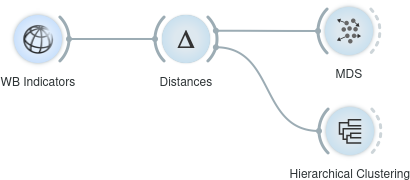
\includegraphics[width=5cm]{pic/clustering_setup.png}
\end{center}
\caption{Postavitev okolja za prikaz gru"cenja.}
\label{clustering_setup}
\end{figure} 

\begin{figure}
\begin{center}
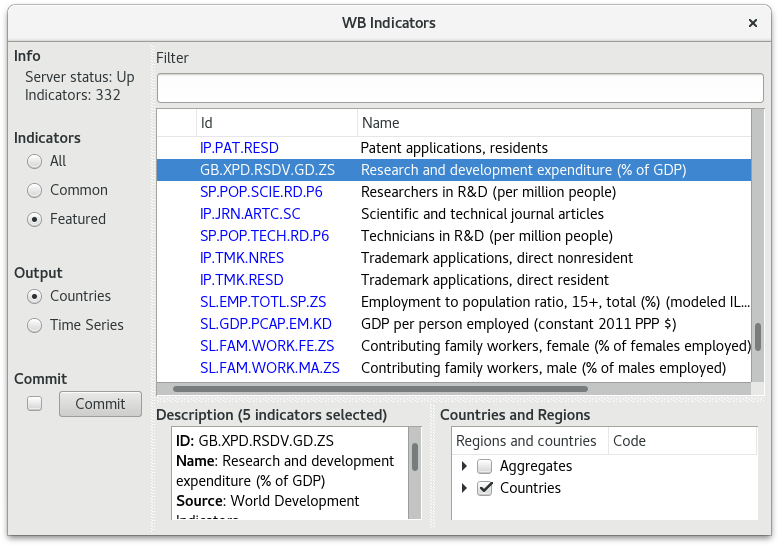
\includegraphics[width=12cm]{pic/clustering_indicator_selection.png}
\end{center}
\caption{Izbor indikatorjev za gru"cenje.}
\label{clustering_indicator_selection}
\end{figure} 

\begin{figure}
\begin{center}
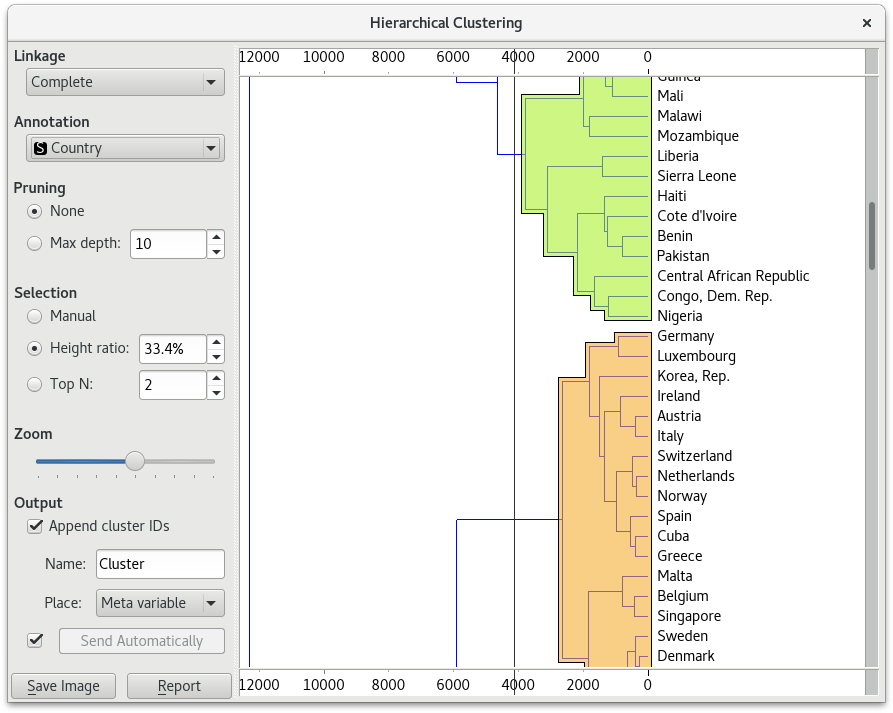
\includegraphics[width=12cm]{pic/clustering_hierarchial_countries.png}
\end{center}
\caption{Prikaz hierarhi"cnega gru"cenja dr"zav.}
\label{clustering_hierarchial_countries}
\end{figure} 

\begin{figure}
\begin{center}
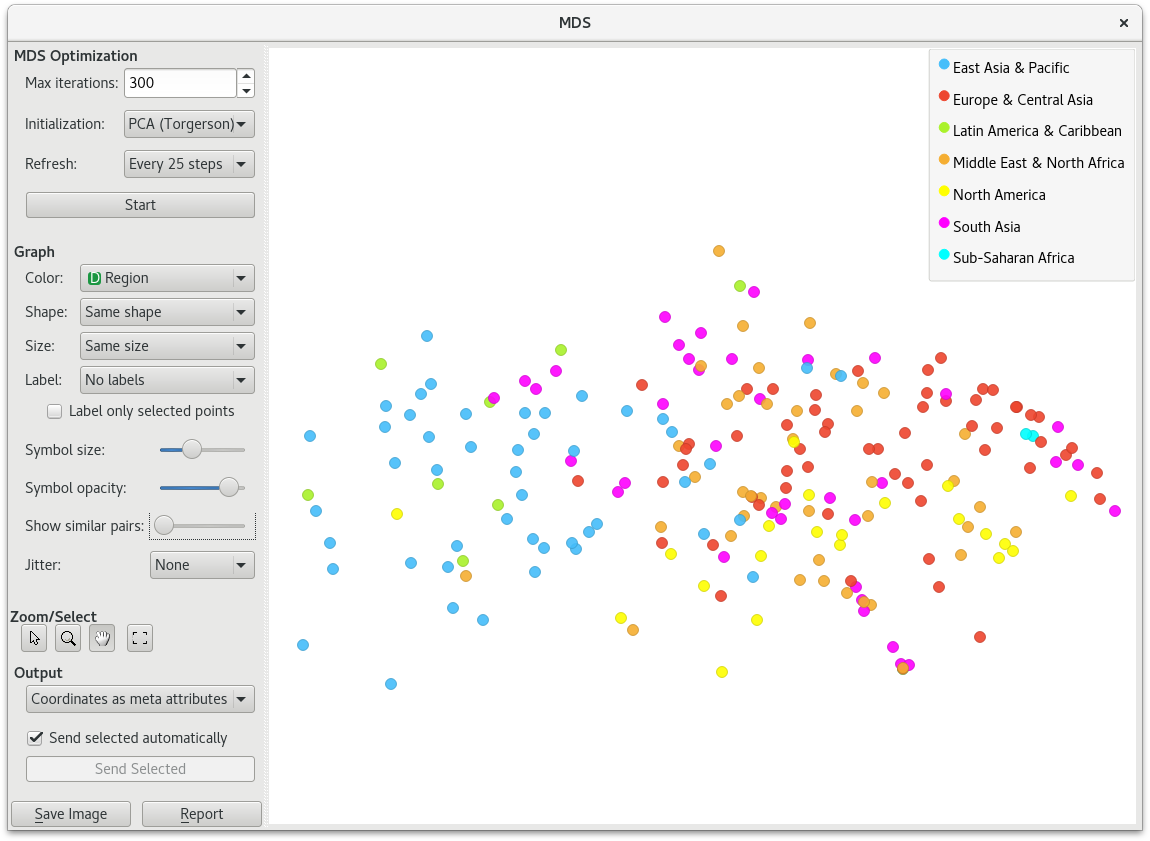
\includegraphics[width=12cm]{pic/clustering_mds.png}
\end{center}
\caption{Prikaz gru"cenja MDS.}
\label{clustering_mds}
\end{figure} 

